% Author: Naomi Sagan, Ryan Koh
% Emails: naomi.sagan@berkeley.edu, ryan_koh@berkeley.edu

\qns{Intro to Discrete-Time Systems}

\usetikzlibrary{calc, automata, chains, arrows.meta}

Students are studying for the EECS16C exam, and the flow of students from Moffit to Taejin's Office Hours (OH) can be represented as the following: \newline

\begin{align*}
    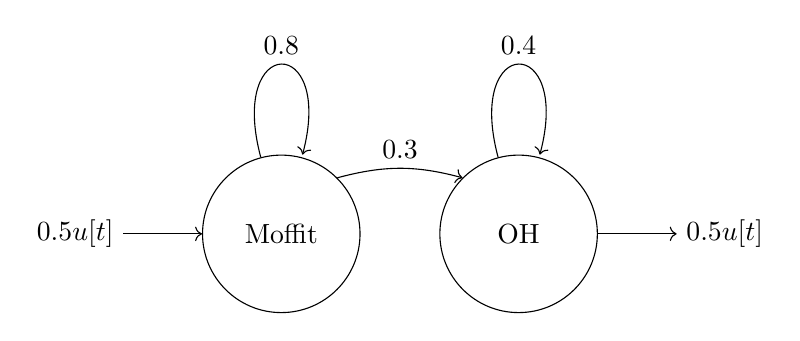
\begin{tikzpicture}
        \node[circle, draw=black, minimum size=2cm] (Moffit) {Moffit};
        \node[circle, draw=black, minimum size=2cm] (OH) [right=of Moffit] {OH};
        \draw [->] (Moffit.north east) to [bend left=15]  node[above] {0.3}  (OH.north west);
        \path (Moffit) edge [loop above] node {0.8} (Moffit);
        \path (OH) edge [loop above] node {0.4} (OH);
        \node (u_moffit) [left=of Moffit] {$0.5u[t]$};
        \draw [->] (u_moffit.east) to []  node[left] {}  (Moffit.west);
        \node (u_OH) [right=of OH] {$0.5u[t]$};
        \draw [<-] (u_OH.west) to []  node[right] {}  (OH.east);
    \end{tikzpicture}
\end{align*}

where $u[t]$ is the number of students that start to study at timestep $t$. (i.e.: $u[t]$ is the input to the system)

\begin{enumerate}
    \qitem Let our state variables be represented by $x_1$ and $x_2$. \textbf{Explain in your own words what $x_1$ and $x_2$ are.}
        \sol{
        }
        \sol{
        }
        \sol{
        }
    \qitem Represent the flow of students between the two states as a matrix-vector discrete time system:
    \begin{align*}
        \vec{x}[t+1] =  A\vec{x}[t] + \vec{b}u[t]\\
    \end{align*}
    \textbf{Find matrix $A$ and vector $\vec{b}$.}
    \sol {
    }

    \qitem Let $\vec{x}[0] = \vec{0}$, and $u[t] = 10$ for all values of $t$. \textbf{What is $\vec{x}[1]$? What is $\vec{x}[2]$?} \textbf{What is $||\vec{x}||$ as $t\rightarrow\infty$? Does that make sense in the context of our problem?}
    

    \sol{
        
    }

    \qitem Let $\vec{x}[0] = \begin{bmatrix} 50 \\ 50 \end{bmatrix}$, and $u[t] = -4$ for all values of $t$. \textbf{What is $\vec{x}[1]$? What is $\vec{x}[2]$?} \textbf{What is $||\vec{x}||$ as $t\rightarrow\infty$? Does that make sense in the context of our problem?}

    \sol{

    }

    \qitem Let $\vec{x}[0] = \vec{0}$, $u[0] = 16$, and $u[t>0] = 0$. \textbf{What is $\vec{x}[1]$? What is $\vec{x}[2]$?} \textbf{What is $||\vec{x}||$ as $t\rightarrow\infty$? Does that make sense in the context of our problem?}

    \sol {

    }
\end{enumerate}